\section[Target]{Target \label{sec:target} }
A schematic diagram of the \gx{} liquid hydrogen cryotarget is shown in Fig.~\ref{fig:Target}. The major components of the system are a pulse tube cryocooler,\footnote{Cryomech model PT415.} a condenser, and a target cell.  These items are contained within an aluminum and stainless steel `L'-shaped vacuum chamber with an extension of closed-cell foam\footnote{Rohacell 110XT, Evonik Industries AG.} surrounding the target cell. In turn, the \gx{} Start Counter (Sec.~\ref{sec:st}) surrounds the foam chamber and is supported by the horizontal portion of the vacuum chamber. Polyimide foils, 100~$\mu$m thick, are used at the upstream and downstream ends of the chamber as beam entrance and exit windows. The entire system, including the control electronics, vacuum pumps, gas-handling system, and tanks for hydrogen storage, are mounted on a small cart that is attached to a set of rails for insertion into the \gx{} solenoid.  To satisfy flammable gas safety requirements, the system is connected at multiple points to a nitrogen-purged ventilation pipe that extends outside Hall D.
\begin{figure*}
\begin{center}
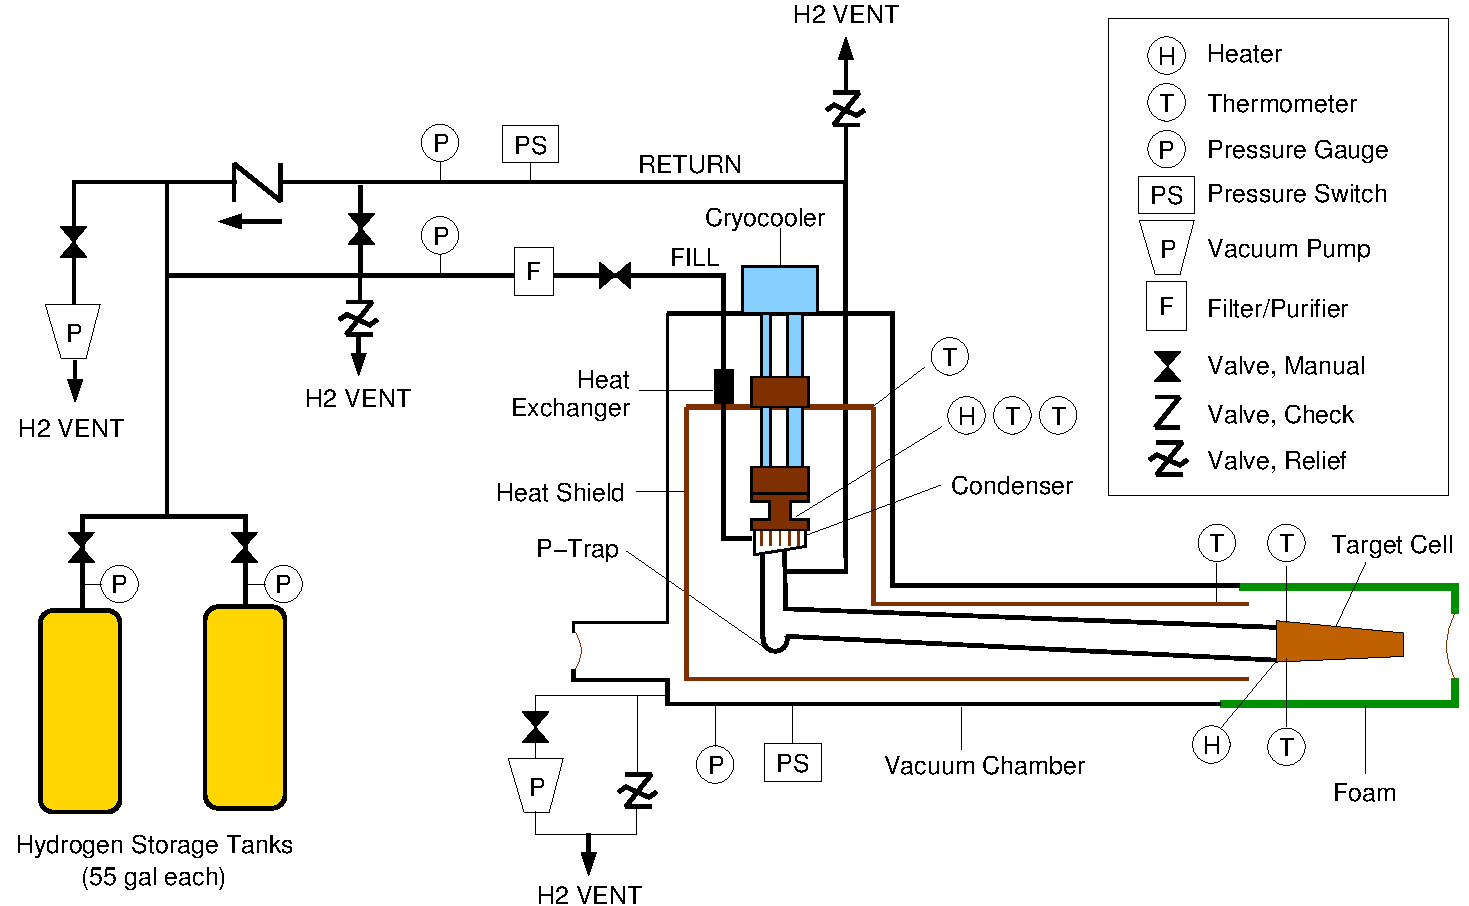
\includegraphics[width=4.5in]{figures/TargetSchematic3.pdf}
\end{center}
\caption{Simplified process and instrumentation diagram for the GlueX liquid hydrogen target (not to scale).
In the real system, the P-trap is above the level of the target cell and is used to
promote convective cooling of the target cell from room temperature.}
\label{fig:Target}
\end{figure*}

Hydrogen gas is stored inside two 200~l tanks and
is cooled and condensed into a small copper and stainless steel container,
the condenser, that is thermally anchored to the second cooling stage of the cryocooler. 
The first stage of the cryocooler is used to
cool the H$_2$ gas to about 50~K before it enters the condenser.
The first stage also cools a copper thermal shield that surrounds all
lower-temperature components of the system except for the
target cell itself, which is wrapped in a few layers of aluminized-mylar/cerex insulation.

The condenser is comprised of a copper C101 base
sealed to a stainless steel can with an indium O-ring.  Numerous vertical 
fins are cut into the copper base, giving a large surface area for condensing hydrogen gas.
A heater and a pair of calibrated Cernox thermometers\footnote{Cernox, Lake Shore Cryotronics.}
are attached outside the condenser, and are used to regulate the heater temperature when the
system is filled with liquid hydrogen.

The target cell, shown in Fig.~\ref{fig:TargetCell}, is similar to
designs used in Hall B at JLab~\cite{HAKOBYAN2008218}.  
The cell walls are made from 100-$\mu$m-thick aluminized
polyimide sheet wrapped in a conical shape and glued along the edge,
overlapping in a 2~mm wide scarf joint.  
The conical shape prevents bubbles from collecting inside the cell, while the
scarf joint reduces the stress riser at the glue joint.  This conical
tube is glued to an aluminum base, 
along with stainless steel fill and return tubes leading to the condenser, a feed-through for two calibrated Cernox thermometers inside the cell, and a
polyamide-imide support for the reentrant upstream beam window.  
Both the upstream and downstream beam
windows are made of non-aluminized,
100~$\mu$m thick polyimide films that have been extruded into the
shapes indicated in Fig.~\ref{fig:TargetCell}. These windows are clearly
visible in Fig.~\ref{fig:z-vertex} where reconstructed vertex positions are shown. All items are glued together using
a two-part epoxy\footnote{3M Scotch-Weld epoxy adhesive DP190 Gray.}
that has been in reliable use at cryogenic temperatures for long periods. 
A second  heater, attached to the aluminum base,
is used to empty the cell for background measurements.
The base is attached to a kinematic mount, which is in turn
supported inside the vacuum chamber using a system of carbon fiber rods.    
The mount is used to correct the pitch and yaw
of the cell, while $X$, $Y$, and $Z$ adjustments 
are accomplished using positioning screws on the target cart. 


During normal operation, a sufficient amount of hydrogen gas is condensed from the storage tanks
until the target cell, condenser, and interconnecting piping are filled with liquid hydrogen
and an equilibrium pressure of about 19~psia is achieved.  
The condenser temperature is regulated at 18~K, while the
liquid in the cell cools to about 20.1~K. The latter temperature is 1~K below the saturation
temperature of H$_2$, which eliminates boiling within the cell and permits a more
accurate determination of the fluid density, 
$71.2 \pm 0.3$~mg/cm$^3$.  
The system can be cooled from room temperature and filled with liquid hydrogen in
approximately six hours.  Prior to measurements using an empty target cell, the liquid hydrogen is boiled back into the storage tanks in about five minutes.  H$_2$ gas continues to condense and drain towards the target cell, but the condensed hydrogen is immediately 
evaporated by the cell heater.  In this way, the cell does not warm above 40~K and
can be re-filled with liquid hydrogen in about twenty minutes.

\begin{figure}
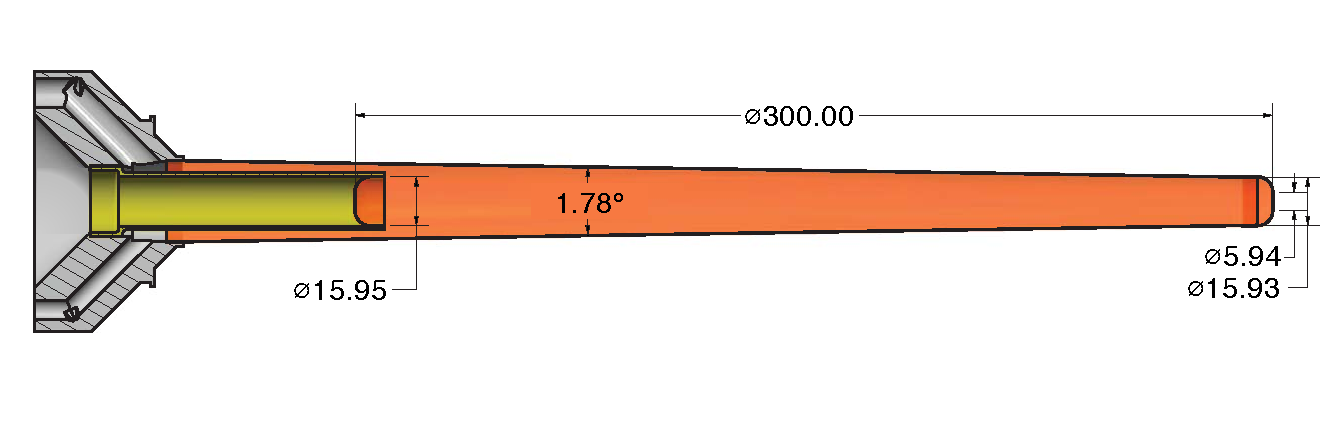
\includegraphics[width=3.5in]{figures/GluexCell_mm.pdf}
\caption{Target cell for the liquid hydrogen target.  Dimensions are in mm.  }
\label{fig:TargetCell}
\end{figure}

Operation of the cryotarget is highly automated, requires minimal user intervention,
and has operated in a very reliable and predictable manner throughout the
experiment. 
The target controls\footnote{The control logic uses National Instruments CompactRIO 9030.} are handled by a LabVIEW program, 
while a standard EPICS softIOC running in Linux provides a
bridge between the controller and JLab's EPICS enviroment (see Section\,\ref{sec:controls}).     
Temperature read back and control of the condenser and target cell thermometers
are managed by a four-input temperature
controller\footnote{Lake Shore Model 336.} with PID control loops of 50 and 100~W.
Strain gauge pressure sensors measure the fill and return pressures with 0.25\% 
accuracy.  When filled with subcooled liquid, 
the long-term temperature ($\pm 0.2$~K) and pressure ($\pm 0.1$~psi)
stability of the liquid hydrogen enable a determination of the density to better than 0.5\%.


